\documentclass{standalone}
\usepackage{graphicx}	
\usepackage{amssymb, amsmath, amsthm}
\usepackage{color}

\usepackage{tikz}
\usetikzlibrary{intersections, backgrounds, math}

\definecolor{light}{RGB}{220, 188, 188}
\definecolor{mid}{RGB}{185, 124, 124}
\definecolor{dark}{RGB}{143, 39, 39}
\definecolor{highlight}{RGB}{180, 31, 180}
\definecolor{darkteal}{RGB}{29, 79, 79}
\definecolor{darkolive}{RGB}{97, 123, 45}
\definecolor{gray10}{gray}{0.1}
\definecolor{gray20}{gray}{0.2}
\definecolor{gray30}{gray}{0.3}
\definecolor{gray40}{gray}{0.4}
\definecolor{gray60}{gray}{0.6}
\definecolor{gray70}{gray}{0.7}
\definecolor{gray80}{gray}{0.8}
\definecolor{gray90}{gray}{0.9}
\definecolor{gray95}{gray}{0.95}

\tikzmath{
  function normal(\x) {
    return exp(-0.5 * \x * \x);
  };
}

\begin{document}

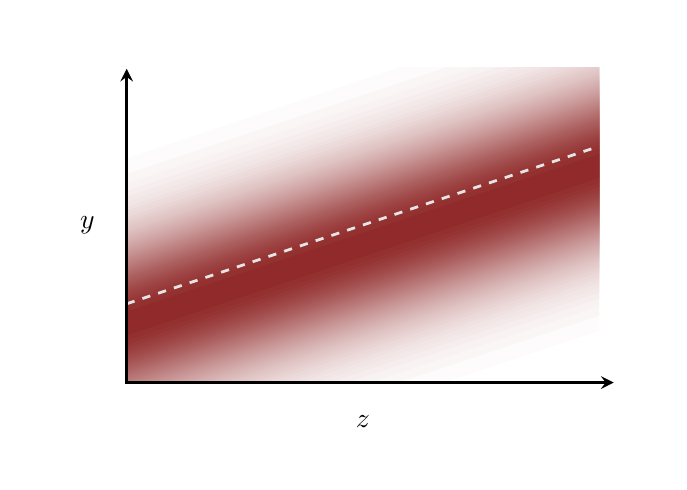
\begin{tikzpicture}[scale=1.0]
  
\begin{scope}[shift={(0, 0)}]
  \draw[white] (-4.25, -3) rectangle (3.75, 2.5); 
  
  \pgfmathsetmacro{\mu}{-0.25}  
  \pgfmathsetmacro{\tau}{0.75}
  \pgfmathsetmacro{\N}{50}
  
  \begin{scope}
    \clip (-3, -2) rectangle (3, 2);
    \foreach \n in {1, ..., \N} {
      \pgfmathsetmacro{\delta}{\tau * sqrt(-2 * ln(\n / \N))}
      \pgfmathsetmacro{\prop}{100 * (\n / \N)}
      \colorlet{custom}{dark!\prop!white};
      \fill[custom] (-3, -1 - \delta + \mu) -- (+3, +1 - \delta + \mu) -- (+3, +1 + \delta + \mu) -- (-3, -1 + \delta + \mu);
    }
  \end{scope}
  
  \draw[gray90, dashed, line width=1] (-3, -1) -- (3, 1);
    
  \draw[->, >=stealth, line width=1] (-3.00, -2.015) -- +(0, 4);
  \draw[->, >=stealth, line width=1] (-3.015, -2.00) -- +(6.2, 0);
  
  \node at (0, -2.5) { $z$ };
  \node at (-3.5, 0) { $y$ };
\end{scope}
  
\end{tikzpicture}

\end{document}  